\section{Comparing Populations}

\subsection{Differences between Means}

\subsubsection{Sampling Distribution of Differences between Means}
\begin{objectives}
    \item Compute mean, standard error, variance of differences of means
    \item Compute the probability of a difference between means being above a specified
    value
    \item Calculate a Confidence Interval of difference between means with a specific confidence level
       \item Test the differences of two means
    \item Calculate t and p for difference of means
\end{objectives}
\vbox{}
For statistical analyses, it is often more important to concern for difference between means. For example, the difference of means of a control group and an experiment group.
The \Index{Sampling Distribution of Difference between Means} can be though of select samples from each population and get their differences of means repeatedly.
\vbox{}
\\Then, naturally we can know \Index{mean of the sampling distribution of the difference
between means} the mean of the distribution of differences between sample means
is equal to the difference between population means
\begin{equation}
    \mu_{M1-M2}=\mu_1-\mu_2
\end{equation}
As for \Index{variance of the sampling distribution of the difference between
means}
\begin{equation}
    {\sigma^{2}}_{M1-M2}={\sigma^{2}}_{M1}+{\sigma^{2}}_{M2}
\end{equation}
the variance of the sampling distribution of the difference between
means is equal to the variance of the sampling distribution of the mean for
Population 1 plus the variance of the sampling distribution of the mean for
Population 2.
\\We can replace the sample's variance with population's variance:
\begin{equation}
    {\sigma^{2}}_M=\frac{\sigma^{2}}{N}
\end{equation}
If the Variance and Sample Sizes are the same, we can simplify the equation to be:
\begin{equation}
    {\sigma^{2}}_{M1-M2}=\sqrt{\frac{2\sigma^2}{n}}
\end{equation}

\paragraph{\textbf{How to calculate the probability of difference of means being above of below a value}}
:This is the same as to calculate the proportion of a normal distribution being above or below a value. We just use the calculator and type in the standard deviation and mean of this distribution and find the proportion.
\begin{figure}[H]
        \centering
            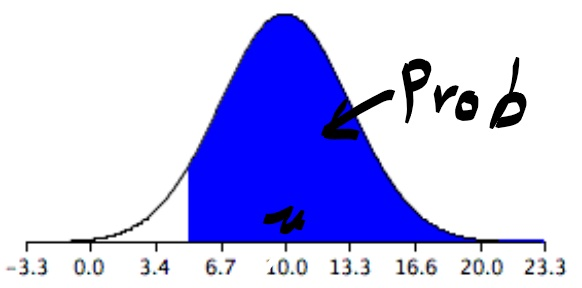
\includegraphics[width=80mm]{prob1.jpg}
            \caption{Probability for being above}
            \label{Probability for being above}
\end{figure}

\textbf{Estimate Confidence Interval}
\\The process is basically the same as calculating the confidence interval for mean of one population. We just have replace several terms.
\\There are three important assumptions for estimating Confidence Interval:
\begin{enumerate}
    \item Variances of the two populations are the same. It's also know as \Index{assumption of homogeneity of variance}.
    \item Difference of means has \textbf{Normal Distribution}.
    \item Every value is independently sampled.
\end{enumerate}
The equation for \Index{Confidence Interval of Difference between Means}:
\begin{equation}
    (M1-M2)\pm (t_{c.l.})(S_{M1-M2})
\end{equation}
\(t_{c.l.}\) should be computed with the calculator using specific \textbf{degrees of freedom}:
\begin{equation}
    d.f.=(n_1-1)+(n_2-1)
\end{equation}
where n is the sample size of two populations
\\ \(S_{M1-M2}\) should be computed with given variance:
\begin{equation}
    S_{M1-M2}=\sqrt{\frac{{\sigma_1}^2+{\sigma_2}^2}{n}}
\end{equation}

\Index{MSE}: The estimate of \(\sigma^2\) which is the assumed same variance of two populations.
\begin{equation}
    MSE=\frac{{\sigma_1}^2+{\sigma_2}^2}{2}
\end{equation}
\Index{SSE}: Sum of squared error. Sometimes the sample sizes of two means are different, and we need SSE:
\begin{equation}
    SSE= \sum\left (x-M1 \right )^{2}+\sum \left ( x-M2 \right )^{2}
\end{equation}

\textbf{Hypothesis Test}
The means of two populations sometimes do not matter, what is important is that if there is actually a difference between the means of populations. 
\\
\begin{examplebox}{Difference between Means}
    If there is a new drug, researchers have to compare the mean of the control group and experiment group. Only the difference actually matters, it's important to know if it exists and how big it is.
\end{examplebox}
\vbox{}
There are three important assumptions for testing if the Difference exists:
\begin{enumerate}
    \item Variances of the two populations are the same. It's also know as \Index{assumption of homogeneity of variance}.
    \item Difference of means has \textbf{Normal Distribution}.
    \item Every value is independently sampled.
\end{enumerate}

The test is just like estimating the probability of rejecting the null hypothesis we learnt before:
\begin{equation}
    t=\frac{(M1-M2)-0}{S_{M1-M2}}
\end{equation}
\(M1=M2\) is the tested statistic, 0 is the hypothesized value(Null Hypothesis)

\textbf{P-value} is just the probability of being greater than the absolute value of t, we compute it using a calculator like before with specific degrees of freedom like we introduced before.
\\After we compute the P-value, we can conclude:
\begin{itemize}
   \item \textbf{If p-value<\(\alpha\), then we reject \(H_0\)}
    \item \textbf{If p-value>\(\alpha\), then we fail to reject \(H_0\)}
\end{itemize}
\begin{Question}
    What is Pooled variance? When do we use it?
\end{Question}

\subsection{All Pairwise Comparisons among Means}
We have to compare more than two means and compare each pair of means. Then as more means being compared, the probability of Type One Error increases. So to eliminate this problem, we introduce the \Index{Tukey HSD test} with \Index{studentized range distribution}.
\begin{examplebox}{All Pairwise Comparison}
    We want to know weather's effect on people's math performance. Then we have to compare sunny, rainy, snowy, windy, and foggy with each other.
\end{examplebox}

\vbox{}
\textbf{Steps of Tukey HSD Test}
\begin{enumerate}
    \item Compute the Variance and Mean for each group
    \item Compute MSE, the mean of variace
    \item Compute Q: 
    \begin{equation}
        Q=\frac{M_i-M_j}{\sqrt{MSE}}
    \end{equation}
    \item Compute P using a specific calculator
\end{enumerate}

\begin{figure}[H]
        \centering
            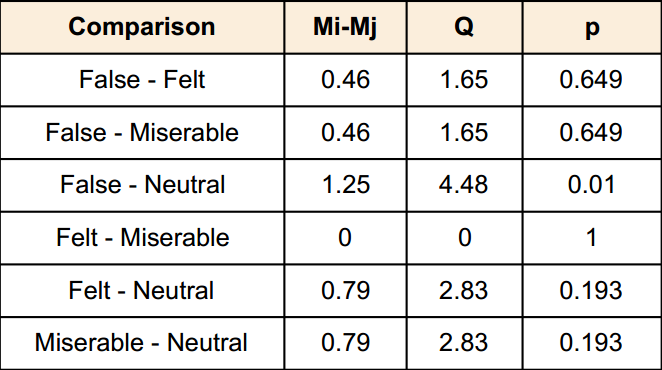
\includegraphics[width=80mm]{Tukey.png}
            \caption{Tukey HSD Test}
            \label{Tukey HSD Test}
\end{figure}
\begin{examplebox}{Tueky Test conclusion}
    For the test result above, what can we conclude?
    \\The false smile is higher than the control
and that the miserable smile is either (a) equal to the false smile, (b) equal to the
control, or (c) somewhere in-between
\end{examplebox}
\subsection{Specific Comparison}
\begin{objectives}
    \item Know Linear Combination
    \item Express Linear Combination with coefficients and means
    \item Do significance test for specific comparison
    \item Know error rates 
\end{objectives}
\vbox{}

Sometimes we have to a more complex comparison between means for more variables, how do we test Significance for the difference?
\\
\begin{examplebox}{More complex comparison}
    We have the scores for students that can be classified as male or female; tall or short. The scores can be compared between the groups with the free combination of gender and length. Through the test, we wish to know which comparison actually make a difference.
\end{examplebox}
\vbox{}
 \textbf{Steps of Test:}
\begin{enumerate}
    \item Express this difference in terms of a linear combination
using a set of coefficients and the means
    \item Compute L-\Index{Linear Combination}: The computation each means times one over total result and add together, same value we got when we computed the difference between means
    \begin{equation}
        L=\sum c_iM_i
    \end{equation}
    where \(c_i\) is the ith coefficient and \(M_i\) is the ith mean
    \item Compute t for testing L for Significance
    \begin{equation}
        t=\frac{L}{\sqrt{\frac{\sum {c_i}^2 MSE}{n}}}
    \end{equation}
    \item Use the calculator to find two-tailed probability and conclude
\end{enumerate}
\begin{Question}
    How do we use L to get p-value? What do we compare p to?
\end{Question}
\vbox{}
\textbf{Multiple comparison}
\\As we add more and more comparison, it's more possible to make Type one error, we need to distinguish two error rates:
\begin{itemize}
   \item \Index{per-comparison error rate}: the probability of a Type I error for a particular comparison.
   \item \Index{familywise error rate(FW)}: the probability of making one or more Type I errors in a family or set of comparisons.
\end{itemize}

\subsection{Correlated Pairs}
\begin{objectives}
    \item Tell if you have Correlated Pairs instead of Independent Group
    \item Do significance test for Correlated Pairs    
\end{objectives}
\vbox{}
Sometimes when we compare means, we cannot compare them with the test we introduce before, because they are not independent. They are related to each other. So they are \Index{Correlated Pairs}, what we discuss before are \Index{Independent Pairs}.
\\
\begin{examplebox}{Correlated Pairs}
     If the experiment is test the effect of a new drug on the disease. The subjects take the new drug or placebo and are measured. There is only one group of subjects,
each subject being tested in both the conditions. The means are correlated.
\end{examplebox}
\vbox{}
\textbf{Steps for test of Correlated Pairs}
\begin{enumerate}
    \item Compute the difference of scores of each subject
    \item Do the test of a single mean for the mean of differences between means.
\end{enumerate}
correlated t tests  have more power than
independent-groups t tests, because standard error of the difference between means is smaller in the correlated t
test and, since this term is in the denominator of the formula for t, results in a
larger t.
